\definecolor{colorOne}{HTML}{443E46}
%\definecolor{colorTwo}{HTML}{F6DEB8}
\definecolor{colorTwo}{HTML}{FFFFFF}

\definecolor{colorThree}{HTML}{908CA4}
\definecolor{colorFour}{HTML}{57659E}
\definecolor{colorFive}{HTML}{C57284}
\definecolor{colorSix}{HTML}{FF5B69}

% Raccourcis pour les couleurs
\def\colorOne{colorOne}
\def\colorTwo{colorTwo}
\def\colorThree{colorThree}
\def\colorFour{colorFour}
\def\colorFive{colorFive}
\def\colorSix{colorSix}

\definecolor{colorGold}{HTML}{FFD700}
\def\colorGold{colorGold}

\usetikzlibrary {decorations.text}
\usetikzlibrary {arrows.meta}


\tikz \fill [decorate,decoration={text along path,
               text=This is a text along a path. Note how the path is lost.}]
  [fill=blue!20,draw=blue,thick] (0,0) -- (2,1) arc (90:-90:.5) -- cycle;


\usetikzlibrary{%
  arrows,%
  calc,%
  shapes.geometric,%
  shapes.misc,%
  shapes.symbols,%
  shapes.arrows,%
  automata,%
  through,%
  positioning,%
  scopes,%
  decorations.shapes,%
  decorations.text,%
  decorations.pathmorphing,%
  shadows}

  \usetikzlibrary{decorations.markings,arrows.meta}
  \usetikzlibrary{intersections}


  % Définition de la fonction pour générer la grille
\newcommand{\drawgrid}[4]{


	\begin{scope}[opacity = 0.2]
	
	
    	% Paramètres : #1=xmin, #2=xmax, #3=ymin, #4=ymax

   	 	% Grille principale en cm
    	\draw[very thin, gray] (#1,#3) grid (#2,#4); % Grille de base (1 cm)
    
    	\draw[very thin, gray] (#1,#3) grid[step=0.1] (#2,#4);

    	\draw[thin, black] (#1,#3) edge[thick,line width=0.8ex,->,>=Stealth ] (#2,#3); 
    
    	\foreach \x in {#1,..., #2} {
        	\draw[shift={(\x, #3)}] (0,-0.1) edge[line width=0.8ex] node[pos = -1 , below] {\x} (0,0.1); % Lignes verticales en mm
    	}

    	\draw[thin, black] (#1,#3)edge[thick,line width=0.8ex,->,>=Stealth ] (#1,#4); 
    
    	\foreach \y in {#3,..., #4} {
        	\draw[shift={(#1, \y)}] (-0.1 , 0 ) edge[line width=0.8ex] node[pos = -1 , left ] {\y} (0.1 , 0); % Lignes verticales en mm
    	}
    
    \end{scope}


}



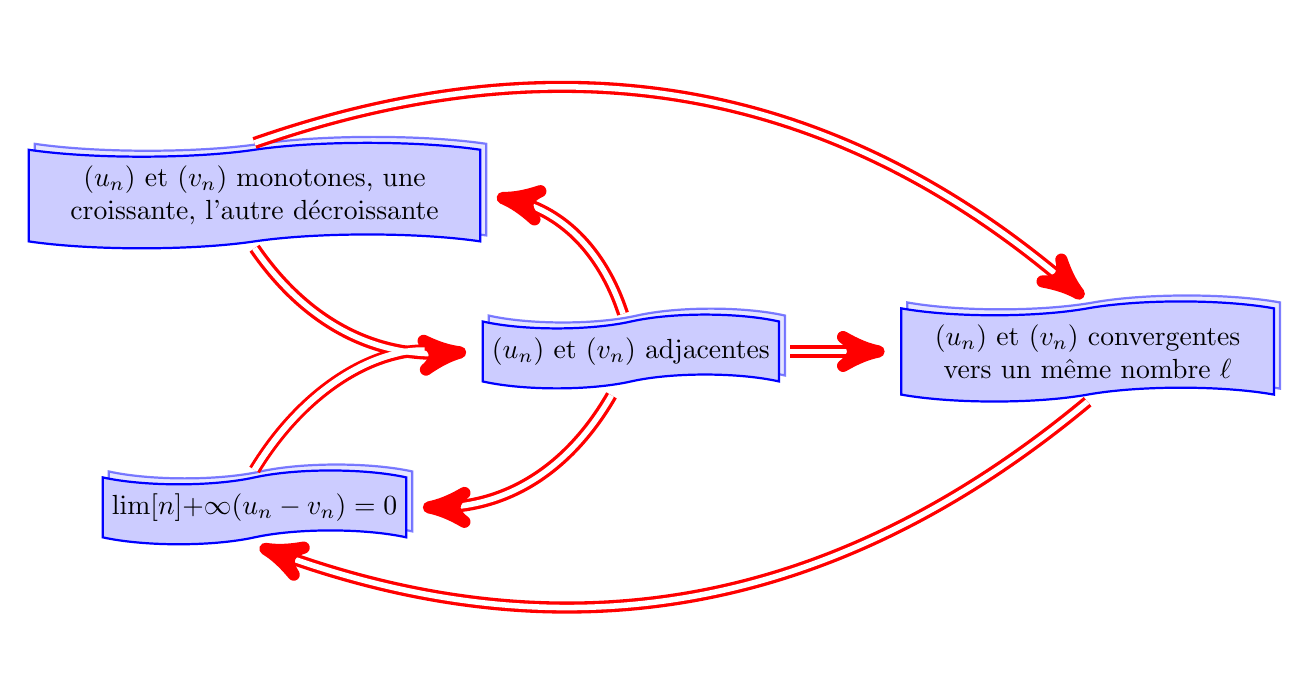
\begin{tikzpicture}[on grid,semithick,node distance=2.8cm,auto,
every state/.style={copy shadow={opacity=.5},tape,outer sep =4pt,
                    fill=blue!20,draw=blue,thick}] 

\tikzset{fleche/.style={->,>=stealth',shorten >=2pt, red,  very thick,double,double distance=2pt}}  
                
\node(O){};
\node[state] (A) [text width=5.5cm,text centered,above left=of O] {$(u_n)$ et $(v_n)$ monotones, une croissante, l'autre décroissante};
\node[state] (B) [below left=of O] {$\lim[n]{+\infty}(u_n-v_n)=0$};
\node[state] (C) [right=of O] {$(u_n)$ et $(v_n)$ adjacentes};
\node[state] (D) [text width=4.5cm,text centered,right=of C,xshift=3cm] {$(u_n)$ et $(v_n)$ convergentes vers un même nombre $\ell$}; 
\draw[fleche] (A.north)  to [bend left] (D.north); 
\draw[fleche] (C.east)to(D.west);
\draw[fleche] (C)to[bend right](A.east); 
\draw[fleche] (C)to[bend left](B.east);
\draw[fleche] (D.south)to[bend left](B.south);
\draw[fleche,-,shorten >=16pt] (B.north)to[bend left](C.west); 
\draw[fleche] (A.south)to[bend right](C.west);
\draw[>=stealth', very thick,white, line width = 2.2pt,-,shorten >=17pt] (B.north)to[bend left](C.west); 
\end{tikzpicture}  

\begin{figure}[H]
	\centering
	\begin{tikzpicture}
		%\begin{scope}[transform canvas={scale=0.6}]
	
		\begin{scope}[shift={(0,0)}]
			
			\node (a) at (0,0) {
        %         \animategraphics[
        %     %controls, 
        %     autoplay, % démarre automatiquement 
        %     %loop, % boucle infinie,
        %     %palindrome, % (optionnel) rejoue à l'envers,
        %     %clicktoshow, % permet de lancer/pause par clic
        %     width=0.3\linewidth,
        %     %buttonsize=1em,
        %     poster=first
        %   ]{60}{figures/00_PreRemInt/frames_2D_positions_animation/frame_}{00001}{00001}
            };
        	\node[above=-0.2cm of a , shift={(-2 , 0)}] {\fontsize{12pt}{14pt}\selectfont \bfseries a)};


                
        %\draw [color = white] (-3,-1) rectangle +(10,2);


        	\node[rectangle , right = -1mm of a] (A) at (1.5,1.5) {
            % \parbox{0.55\linewidth}{       
            %     \animategraphics[
            %      autoplay,
            %     %loop,
            %     width=\linewidth,
            %      buttonsize=1em,
            %      poster=first
            %    ]{60}{figures/00_PreRemInt/frames_2D_velocity_distribution/frame_}{00001}{00001}
            %  }
          };
            \node[] at (A) {\fontsize{12pt}{14pt}\selectfont \bfseries (A)};

        %   \node[rectangle , right = -1mm of A ] (B)
        %   {\fontsize{10pt}{5pt}\selectfont 
        %     $ \overset{thermalisation}{\Longrightarrow} $
        %   };

          \node[rectangle , right = 5cm of A  ] (C)  { %at (6,1.5)
            % \parbox{0.55\linewidth}{
            % 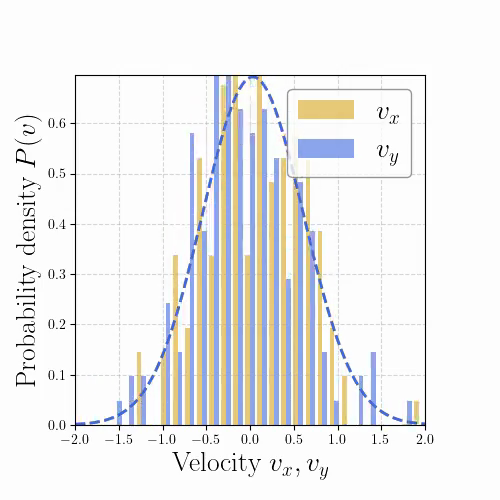
\includegraphics[width=1\linewidth]{figures/00_PreRemInt/frames_2D_velocity_distribution/frame_00600}
            % }
          };

          \node[] at (C) {\fontsize{12pt}{14pt}\selectfont \bfseries (C)};

%          \filldraw[
%     decorate,
%     decoration={text along path, text={Thermalisation.}, text align=center},
%     fill=blue!20,
%     draw=blue,
%     thick
%   ]
%   (A) to[out=90,in=90] (C);

% $\Rightarrow$

% \draw[
%      		decoration={
% 			markings,
%     		mark connection node=my node,
%     		mark=at position .5 with{\node [blue,transform shape] (my node) {\fontsize{10pt}{5pt}\selectfont \bf \color{\colorFour}  $\delta I $};},
%     		%mark=at position 0.1  with {\arrow[blue, line width=0.5ex]{<}},
%     		%mark=at position 1  with {\arrow[blue, line width=0.5ex]{>}}
%     		},
%         	color=\colorThree,
%         	thick,
%         	line width=0.5ex,
%             double equal sign distance,
%             double distance=0.5ex , 
%         	%arrows={Computer Modern Rightarrow[line cap=round]-Computer Modern Rightarrow[line cap=round]}
%    			] %(A) edge[{Computer Modern Rightarrow[line cap=round]}-{Computer Modern Rightarrow[line cap=round]} , out=90,in=90 ]  (C)
%             (A) edge[{Computer Modern Rightarrow[line cap=round]}-{Computer Modern Rightarrow[line cap=round]} , out=90,in=90 ]  (C)
%             %(A) edge[arrows={Computer Modern Rightarrow[line cap=round]-}] ($(A)+(0.1,0.1)$)  decorate {(A) edge[{Computer Modern Rightarrow[line cap=round]}-{Computer Modern Rightarrow[line cap=round]} , out=90,in=90 ] (C)} ($(C)+(-0.1,0.1)$) edge[arrows={-Computer Modern Rightarrow[line cap=round]}] (C)
%             %(A) edge[arrows={Computer Modern Rightarrow[line cap=round]-}] ($(A)+(0.1,0.1)$)decorate {($(A)+(0.1,1.1)$) to[out=90,in=90] ($(C)+(-0.1,0.1)$)}($(C)+(-0.1,0.1)$) edge[arrows={-Computer Modern Rightarrow[line cap=round]}] (C)
%     		;	

\newcommand{\curve}{(A) to[out=90,in=90] (C)} 

\tikzset{fleche/.style={->,>=stealth',shorten >=2pt, red,  very thick,double,double distance=20pt}} 

%\draw[fleche] \curve ;

\draw[
  ->,
  >=Computer Modern Rightarrow,
  trim left=1pt,
  trim right=1pt,
  line width=0.5ex,
  red
] \curve ;


% % Dessin d'une partie du chemin seulement
% \draw[fleche,
%   thick,
%   postaction={
%     decorate,
%     decoration={
%       markings,
%       mark=between positions 0.25 and 0.75 step 1
%       with {
%         \draw[
%           <->,
%           >=Computer Modern Rightarrow
%         ] (0,0) -- (1pt,0);
%       }
%     }
%   }
% ]
%   (A) to[out=90,in=90] (C);

% \draw [decorate,decoration={text along path,
%                text=Thermalisation., pre length=1cm} , draw = none  , red ] (A) to[out=90,in=90] (C);

%             \draw [red] decorate[decoration={text along path,
%                text=Thermalisation., pre length=1cm} , draw = none  , red ]{(A) to[out=90,in=90] (C)} ;

\draw[
  decorate,
  decoration={
    text along path,
    %reverse path,
    text align=center,
    text color=red, % couleur par défaut
    %font=\sffamily\fontsize{10pt}{12pt}\selectfont\bfseries,
    text={
      {
         |\sffamily\fontsize{20pt}{12pt}\selectfont\bfseries| Thermalisation || .
      }
    },
    %pre length=1cm
  },
  draw=none
]
(A) to[out=90,in=90] (C);


        	
        \end{scope}

        
	\end{tikzpicture}
	\caption{a) Profil de densité d’un nuage atomique initialement à l’équilibre dans un piège harmonique avec $\omega_\perp = 2 \pi \times  2.6~\mathrm{kHz}$ et $\omega_\parallel = 2 \pi \times 5~\mathrm{Hz}$ (jaune). La courbe grise représente le profil parabolique attendu à l’état fondamental dans le régime \gls{qBEC}, décrit par l’équation d’état $n(x) = [\mu - V_\parallel(x)]/g$. La courbe noire en pointillés correspond à un ajustement des données expérimentales en supposant que le système soit bien décrit par un ensemble thermique (\gls{TBA} (Sec. \ref{chap4:sec:TBA})). Cet ajustement permet d’extraire une température $T = 90~\mathrm{nK}$ et un potentiel chimique $\mu/k_B = 49~\mathrm{nK}$.
	(b1) Profils de densités pour différents centres de sélection $x_0$ représentés sur la Fig.\ref{fig:selection}(b). Les sélections sont de taille $\ell = 37\, \mu m$ et les profils obtenus après un temps d’expansion $\tau =  40 \, ms$. Pour comparer les résultats à une distribution de rapidités, les profils de densités sont multipliés par le rapport $\tau/ \ell$ et sont tracés en fonction de $(x-x_0)/\tau$. (b2) Prédiction théorique de la distribution de rapidités spatialement résolue $\rho ( x , \theta)$ à l’équilibre thermique dans un potentiel harmonique longitudinal avec $\omega_\parallel = 2 \pi \times 5~\mathrm{Hz}$. La température $T$ et le potentiel chimique $\mu$ utilisés sont ceux obtenus à partir du profil in situ (a).}
	\label{fig:expansion}
\end{figure}